Table \ref{tab:lead_temp_rise} depicts the relationship between lead length and temperature rise, as presented by Aboyewa \cite{aboyewa2021}.

\begin{table}[H]
    \centering
    \renewcommand{\arraystretch}{1.2}
    \setlength{\tabcolsep}{10pt}
    \begin{tabular}{|c|c|}
        \hline
        \textbf{Lead Length (cm)} & \textbf{Temperature Rise ($^{\circ}$C)} \\
        \hline
        5  & 0.3 \\
        10 & 0.7 \\
        13 & 1.2 \\
        15 & 2.5 \\
        20 & 3.8 \\
        \hline
    \end{tabular}
    \caption{Temperature rise as a function of lead length under MRI. Adapted from Aboyewa, 2021 \cite{aboyewa2021}.}
    \label{tab:lead_temp_rise}
\end{table}


%-------------------------------------------------



\begin{figure}[H]
    \centering
    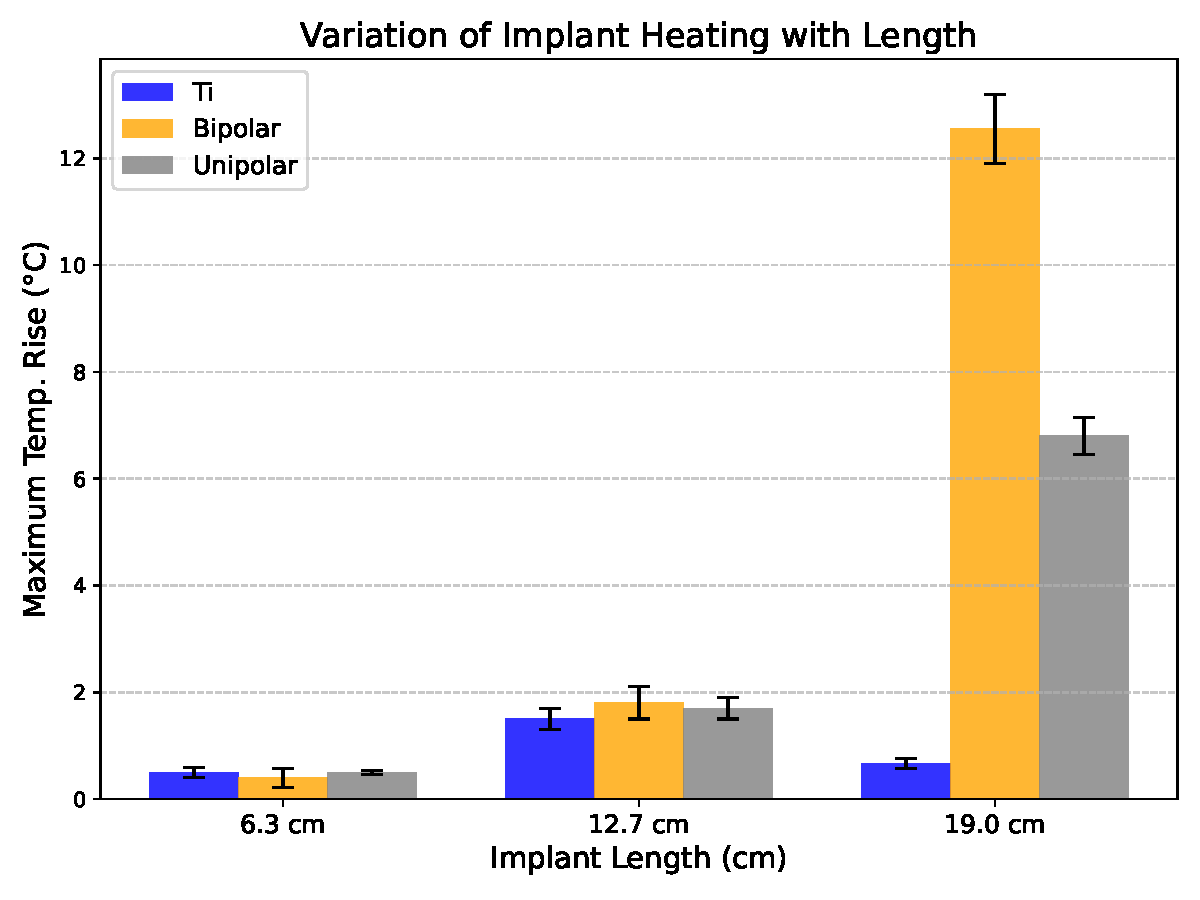
\includegraphics[width=0.8\linewidth]{Figure_4_8_Implant_Heating_Length_With_Errors.pdf}
    \caption{Heating increases with lead length Adapted (Aboyewa, 2021).}
    \label{fig:implant_heating_length}
\end{figure}



%---------------------------------------------------